% chktex-file 44

\documentclass[a4paper,11pt]{article}
\usepackage[utf8]{inputenc}
\usepackage[russian]{babel}
\usepackage{geometry}
\usepackage{amsthm}
\usepackage[dvipsnames]{xcolor}
\usepackage{framed}
\usepackage{booktabs}
\usepackage{array}
\usepackage{amssymb}
\usepackage{adjustbox}
\usepackage{makecell}
\usepackage{float}
\usepackage{graphicx}
\usepackage{amsmath}
\usepackage{physics}
\usepackage{hyperref}
\usepackage{color}
\usepackage{listings}

\definecolor{shadecolor}{RGB}{245,245,247}
\geometry{left=2cm, right=2cm, top=2cm, bottom=2cm}

\title{Модель №.3. \\ Оптика. Кольца Ньютона }
\author{Ким В.Р., Вишневский С.А \\ Группа M3207 }
\date{}

\theoremstyle{definition}
\newtheorem*{task}{Задание}\setlength{\parindent}{0pt}

\newenvironment{solution}
{\begin{shaded}
     \textbf{Решение:}\par\setlength{\parindent}{0pt}}
     {
\end{shaded}}

\newenvironment{answer}
{\par\noindent\textbf{Ответ:} }
{\par}

\definecolor{codegreen}{rgb}{0,0.6,0}
\definecolor{codegray}{rgb}{0.5,0.5,0.5}
\definecolor{codepurple}{rgb}{0.58,0,0.82}
\definecolor{backcolour}{rgb}{0.95,0.95,0.92}

\lstdefinelanguage{MyPython}{
  language=Python,
  morekeywords={np, plt, self, cos, sin},
  sensitive=true,
}
\lstdefinestyle{mystyle}{
    backgroundcolor=\color{backcolour},
    commentstyle=\color{codegreen},
    keywordstyle=\color{magenta},
    numberstyle=\tiny\color{codegray},
    stringstyle=\color{codepurple},
    basicstyle=\ttfamily\footnotesize,
    breakatwhitespace=false,
    breaklines=true,
    captionpos=b,
    keepspaces=true,
    numbers=left,
    numbersep=5pt,
    showspaces=false,
    showstringspaces=false,
    showtabs=false,
    tabsize=2,
    columns=fullflexible,
}

\lstset{style=mystyle}

\begin{document}
    \maketitle

    \begin{task}
        Моделирование колец Ньютона для линзы заданного радиуса.
        Рассмотреть \textit{монохроматический} и \textit{квазимонохроматический} свет
        (задается середина и ширина спектра в нанометрах). Вывод цветного
        распределения интенсивности интерференционной картины и графика
        зависимости интенсивности от радиальной координаты.
    \end{task}


    \section{Теория}

    \subsection{Введение}
    Кольца Ньютона — это интерференционная картина в виде концентрических светлых
    и тёмных колец, наблюдаемая при освещении системы <<выпуклая линза на плоской пластине>> светом.
    Возникает она в результате \textit{интерференции}*** отражённого света в тонком воздушном зазоре между
    поверхностями линзы и пластины. Толщина зазора зависит от расстояния от точки касания,
    поэтому фаза отражённого света изменяется по радиусу, формируя характерные кольца.

    Целью моделирования является вычисление и визуализация распределения интенсивности отражённого света
    в зависимости от радиальной координаты, как для \textit{монохроматического}**, так и для
    \textit{квазимонохроматического}** освещения.
    \\
    \\
    * \textbf{интерференция} — взаимное увеличение или уменьшение результирующей амлитуды двух или нескольких
    когерентных**** волн при их наложении друг на друга
    \\
    \\
    ** \textbf{монохроматический свет} — это световые колебания одной частоты.
    \\
    \\
    *** \textbf{квазихроматический свет} можно представить как суперпозицию монохроматических волн, частоты которых
    расположены в узком спектральном диапазоне.
    \\
    \\
    **** \textbf{когерентные волны:} если частоты колебаний в обеих волнах одинаковы, а разность фаз возбуждаемых колебаний
    остается постоянной во времени, то такие волны называются когерентными.

    \subsection{Геометрия системы}
    Рассматривается выпуклая линза с радиусом кривизны \( R \), которая лежит
    на плоской стеклянной пластине. Между ними образуется тонкий воздушный зазор переменной
    толщины. Вблизи центра (при \( h \ll R \)) толщина зазора \( h(r) \) описывается:
    \begin{equation}
        h(r) = \frac{r^2}{2R}\label{eq:equation}
    \end{equation}

    где:
    \begin{itemize}
        \item \( r \) — расстояние от центра контактной точки (в метрах),
        \item \( R \) — радиус кривизны линзы (в метрах),
        \item \( h(r) \) — толщина воздушного слоя.
    \end{itemize}

    \subsection{Интерференция света}
    Свет отражается от двух границ: верхней (линза–воздух) и нижней (воздух–пластина).
    В результате возникают две когерентные волны, интерферирующие между собой.

    \subsubsection{Разность хода}
    Разность оптических путей между двумя отражёнными волнами:
    \begin{equation}
        \Delta = 2h(r) + \frac{\lambda}{2}\label{eq:equation2}
    \end{equation}

    где \( \lambda \) — длина волны света, а \( \lambda/2 \) — поправка на сдвиг фазы при отражении от более плотной среды.

    \subsubsection{Условия интерференции}

    Для тёмных колец (минимум интенсивности):

    \begin{gather}
        2h(r) = (2m + 1)\frac{\lambda}{2}, \quad m = 0, 1, 2, \dots\\
        r_m = \sqrt{(2m + 1)\frac{\lambda R}{2}}\\
    \end{gather}

    Для светлых колец (максимум интенсивности):

    \begin{gather}
        2h(r) = m \lambda\\
        r_m = \sqrt{m \lambda R}\\
    \end{gather}

    где \( m \) — порядок интерференции.

    \subsection{Интенсивность отражённого света}
    Интенсивность отражённого света рассчитывается как:

    \begin{equation}
        I(r) = I_0 \cdot \left[1 + \cos\left(\frac{2\pi \Delta}{\lambda} \right)\right]\label{eq:equation3}
    \end{equation}

    Подставляя разность хода:

    \begin{equation}
        I(r) = I_0 \cdot \left[1 + \cos\left(\frac{4\pi h(r)}{\lambda} + \pi \right)\right]\label{eq:equation4}
    \end{equation}

    С учётом \( \cos(x + \pi) = -\cos(x) \):

    \begin{equation}
        I(r) = I_0 \cdot \left[1 - \cos\left(\frac{4\pi h(r)}{\lambda} \right)\right]\label{eq:equation5}
    \end{equation}

    И, подставляя \( h(r) \):

    \begin{equation}
        I(r) = I_0 \cdot \left[1 - \cos\left(\frac{2\pi r^2}{\lambda R} \right)\right]\label{eq:equation6}
    \end{equation}

    \subsection{Квазимонохроматический свет}
    При освещении светом с конечной спектральной шириной \( \Delta\lambda \), свет состоит из диапазона
    длин волн, распределённых вокруг центрального значения \(\lambda_0\) : \( \lambda_i \in [\lambda_0 - \Delta\lambda/2, \lambda_0 + \Delta\lambda/2] \).
    Интенсивность отражения тогда определяется усреднением по спектру:

    \begin{equation}
        I(r) = \frac{1}{N} \sum_{i=1}^{N} \left[1 - \cos\left( \frac{2\pi r^2}{\lambda_i R} \right) \right] \cdot S(\lambda_i)\label{eq:equation7}
    \end{equation}

    где \( S(\lambda) \) - вклад каждой длины волны \(\lambda\), он определяется спектральной плотностью,
    распределенной по Гауссу:

    \begin{equation}
        S(\lambda) = \exp\left( -\frac{(\lambda - \lambda_0)^2}{2\sigma^2} \right), \quad \sigma = \frac{\Delta\lambda}{2\sqrt{2 \ln 2}}\label{eq:equation8}
    \end{equation}

    \subsection{Цветовое изображение интерференционной картины}
    Для двумерной визуализации кольцевой структуры строится двумерное поле интенсивности:

    \begin{equation}
        I(x, y) = I\left( \sqrt{x^2 + y^2} \right)\label{eq:equation9}
    \end{equation}

    \subsection{Итоги}
    На основе этой теории можно:
    \begin{itemize}
        \item Рассчитать радиусы тёмных и светлых колец;
        \item Построить зависимость интенсивности от расстояния \( r \);
        \item Получить цветное изображение интерференционной картины;
        \item Исследовать влияние спектральной ширины на чёткость колец.
    \end{itemize}

%   ----------------------------------

    \newpage
    \section{Моделирование}

    В данном разделе описывается структура программы, реализующей моделирование колец Ньютона

    \subsection{Пользовательский интерфейс и настройка параметров}
    В этой части кода реализован графический интерфейс пользователя на базе \texttt{Tkinter}.
    Интерфейс позволяет задать следующие параметры:
    \begin{itemize}
            \item Радиус кривизны \( R \) (м).
            \item Центральная длина волны \( \lambda_0 \) (нм), которая затем переводится в метры.
            \item Ширина спектра \(\Delta \lambda\) (нм), также переводимая в метры.
    \end{itemize}

    \subsection{Расчёт интенсивности}
    Программа рассчитывает интенсивность интерференционной картины в зависимости от радиальной координаты \( r \).
    Для этого используются две функции:
    \begin{itemize}
        \item \textbf{Монохроматический свет:} Функция \texttt{intensity\_mono} рассчитывает интенсивность
        по формуле (9), где \(I_0\) представлена коэффициентом нормировки (в коде установлено значение 0.5).
        Значение выражения \(1 - \cos(\cdot)\) изменяется от 0 до 2, поскольку
        \(\
            \cos\left(\frac{2\pi r^2}{\lambda R}\right) \in [-1, 1].
        \)
        Если принять \(I_0 = 0.5\), то получим
        \[
            I(r) = 0.5\left[1 - \cos\left(\frac{2\pi r^2}{\lambda R}\right)\right],
        \]
        что нормирует интенсивность в диапазон [0, 1]. Такой выбор удобен для визуализации, так как после масштабирования
        (например, перемножением на 255) можно получить корректное 8-битное изображение, где 0 соответствует полной
        темноте, а 255 --- максимальной яркости.

        \begin{lstlisting}[language=MyPython, label={lst:lstlisting}]
        def intensity_mono(self, r, wavelength):
            return 0.5 * (1 - np.cos(2 * np.pi * r ** 2 / (wavelength * self.R)))
        \end{lstlisting}

        \item{\textbf{Квазимонохроматический случай. Усреднение с использованием спектральной плотности}}
        При квазимонохроматическом освещении свет рассматривается как диапазон длин волн
        \[
        \lambda_i \in \left[\lambda_0 - \frac{\Delta\lambda}{2}, \, \lambda_0 + \frac{\Delta\lambda}{2}\right],
        \]
        распределённых вокруг центрального значения \(\lambda_0\). Теоретически интенсивность
        определяется по формуле (13), где \(S(\lambda)\) задаётся Гауссовой функцией (14)

        В реализации используется следующий подход:
        \begin{itemize}
            \item Выбирается 20 равномерно распределённых точек в указанном диапазоне длин волн.
            \item Для каждой длины волны вычисляется вклад (вес) \( S(\lambda) \) с помощью функции
            \texttt{spectral\_density}.
            \item Весовые коэффициенты нормируются так, чтобы их сумма была равна 1. Это необходимо,
            чтобы итоговое усреднение не зависело от числа дискретных точек.
            \item Итоговая интенсивность вычисляется как сумма произведений интенсивности для каждой длины
            волны (рассчитанной по функции \texttt{intensity\_mono}) и соответствующего весового коэффициента.
        \end{itemize}

        Таким образом, формула расчёта интенсивности в коде принимает вид:
        \[
        I_{\text{quasi}}(r) = \sum_{i=1}^{20} w_i \, I_{\text{mono}}(r, \lambda_i),
        \]
        где
        \[
        w_i = \frac{S(\lambda_i)}{\sum_{j=1}^{20} S(\lambda_j)}.
        \]

        \begin{lstlisting}[language=MyPython,label={lst:lstlisting2}]
        def spectral_density(self, wavelength):
            sigma = self.delta_lambda / (2 * np.sqrt(2 * np.log(2)))
            return np.exp(-((wavelength - self.lambda0) ** 2) / (2 * sigma ** 2))

        def intensity_quasi(self, r):
            wavelengths = np.linspace(self.lambda0 - self.delta_lambda / 2,
                                      self.lambda0 + self.delta_lambda / 2, 20)
            total = np.zeros_like(r)
            weights = np.zeros_like(wavelengths)
            for i, wl in enumerate(wavelengths):
                    weights[i] = self.spectral_density(wl)
            # normalising
            weights /= np.sum(weights)

            for wl, weight in zip(wavelengths, weights):
                total += weight * self.intensity_mono(r, wl)
            return total
        \end{lstlisting}
    \end{itemize}


    \subsection{Построение двумерного поля интенсивности}
    Для визуализации интерференционной картины создаётся двумерная координатная сетка, где интенсивность \( I(x,y) \)
    определяется как функция \( I\left(\sqrt{x^2+y^2}\right) \). Это соответствует преобразованию теоретической
    зависимости \( I(r) \) в изображение, что позволяет получить кольцевую структуру модели.

    \begin{lstlisting}[language=MyPython,label={lst:lstlisting3}]
        x = np.linspace(-0.01, 0.01, self.size)
        y = np.linspace(-0.01, 0.01, self.size)
        xx, yy = np.meshgrid(x, y)
        r = np.sqrt(xx ** 2 + yy ** 2)
    \end{lstlisting}

    \subsection{Преобразование интенсивности в изображение и цветовое отображение}
    После расчёта интенсивности выполняется нормировка и преобразование полученных значений в изображение:
    \begin{itemize}
        \item Значения интенсивности умножаются на 255 для перевода в 8-битное представление.
        \item В случае монохроматического света реализуется функция \texttt{wavelength\_to\_rgb},
        которая приближённо преобразует длину волны в соответствующий RGB-цвет. Это упрощение сделано
        для наглядного отображения спектральных характеристик, так как теория не диктует конкретный
        алгоритм преобразования спектра в цвет.
    \end{itemize}


    \section{Демо-примеры запуска программы}
    \subsection{Монохром, близкий к ИК}
    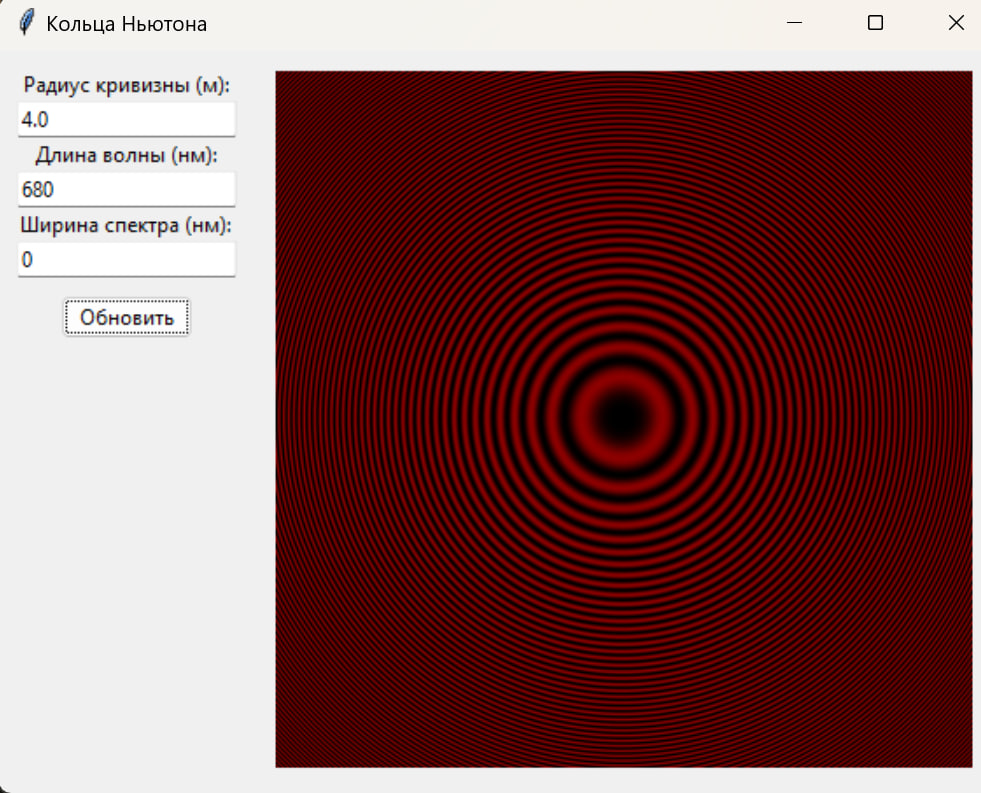
\includegraphics[scale=0.7]{demo results/infraRed_mono}

    \subsection{Монохром, близкий к УФ}
    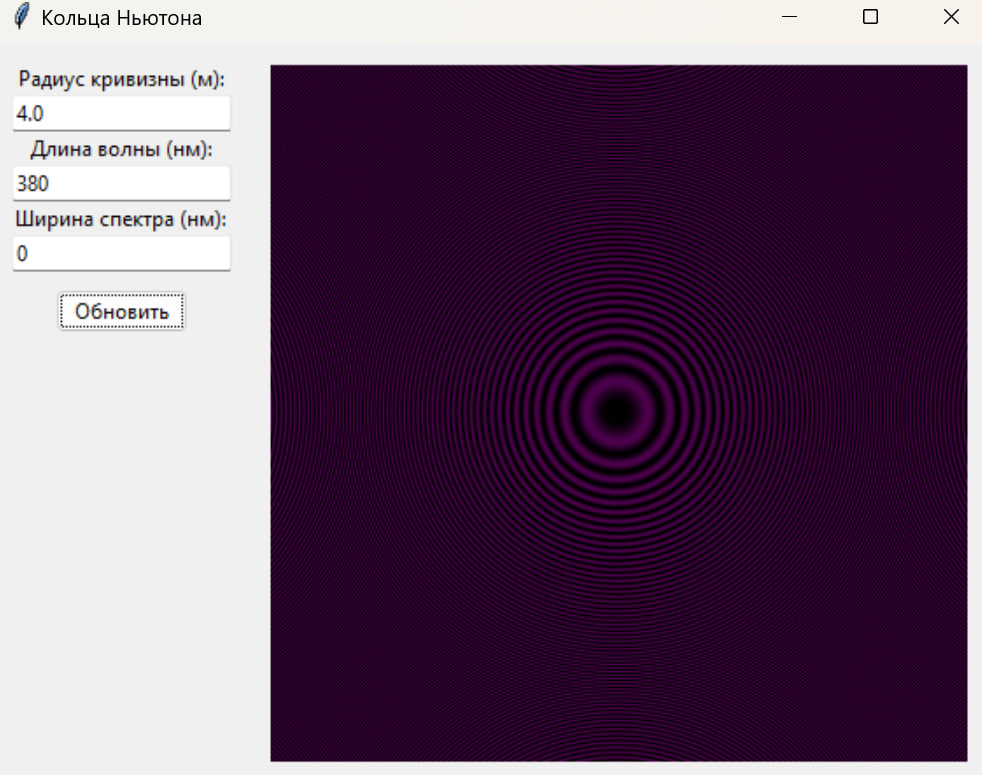
\includegraphics[scale=0.7]{demo results/ultraViolet_mono}

    \subsection{Зеленый монохром}
    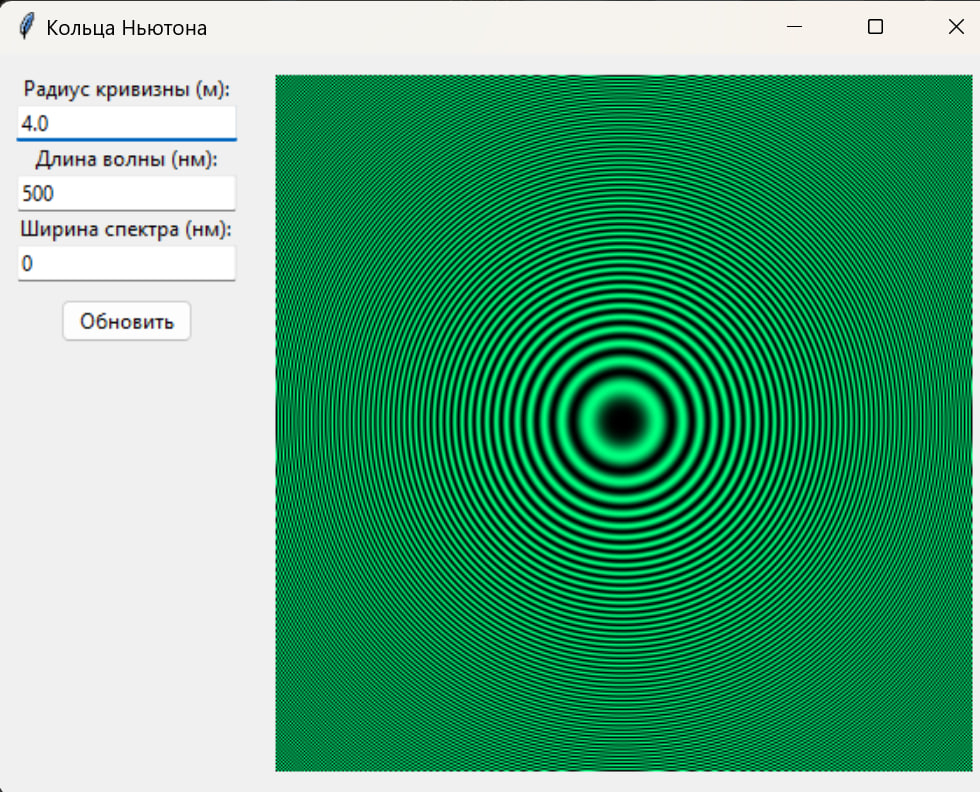
\includegraphics[scale=0.7]{demo results/green_mono}

    \subsection{Большой квазихром}
    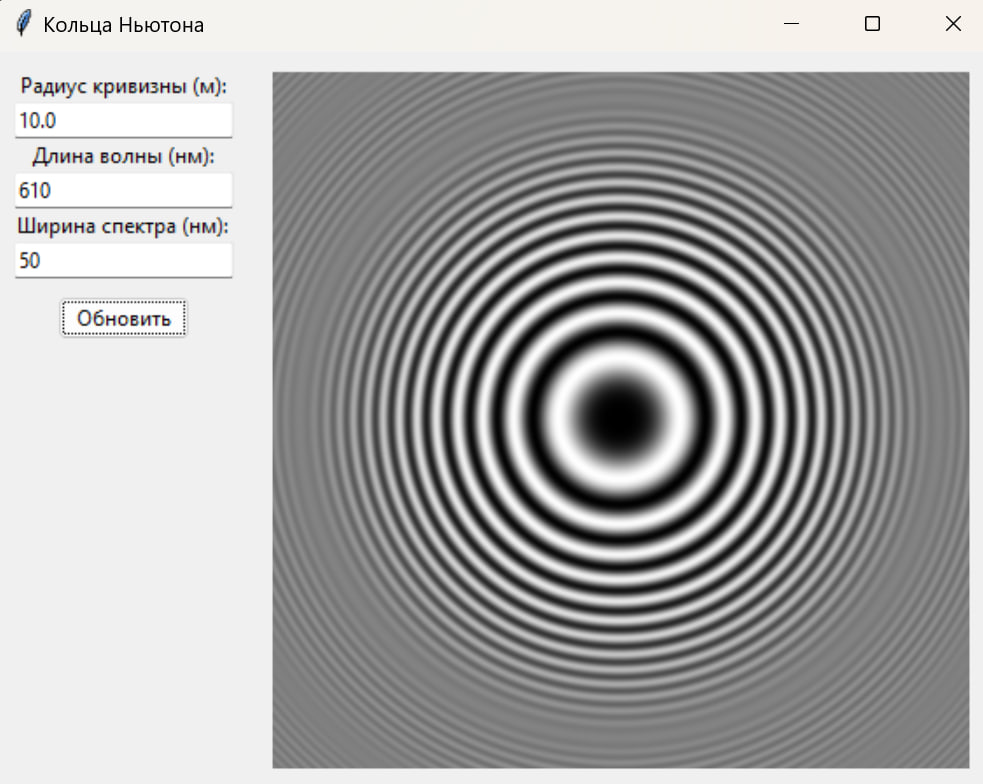
\includegraphics[scale=0.7]{demo results/big_quasi}

    \subsection{Маленький квазихром}
    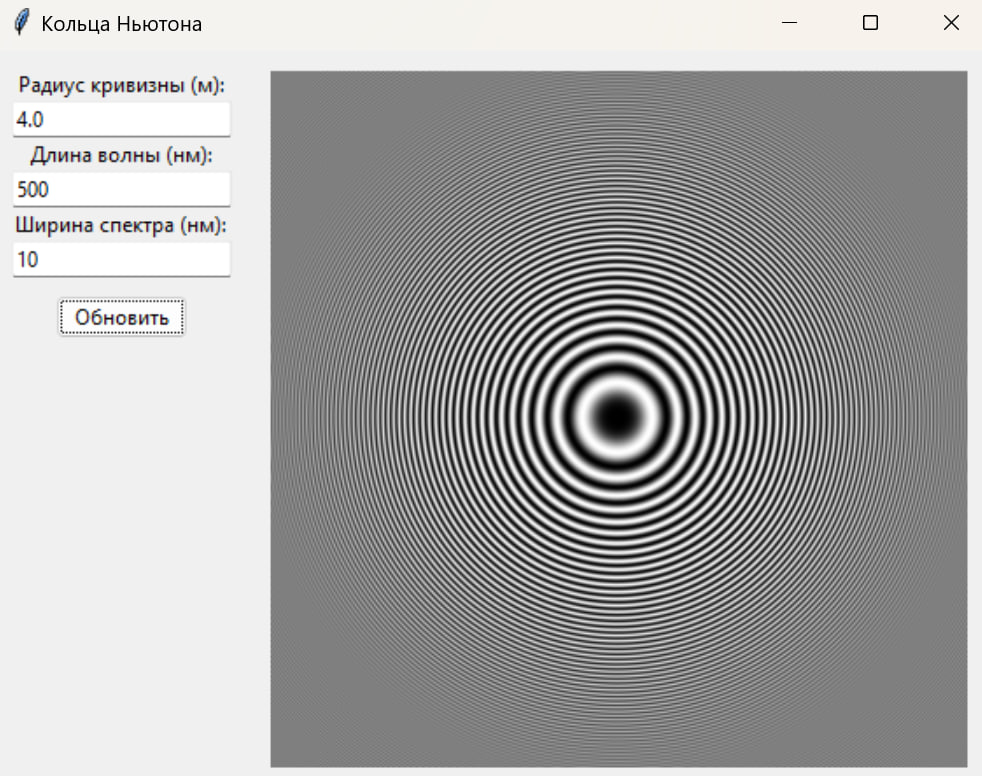
\includegraphics[scale=0.7]{demo results/small_quasi}

    \subsection{Квазихром с широким спектром волн}
    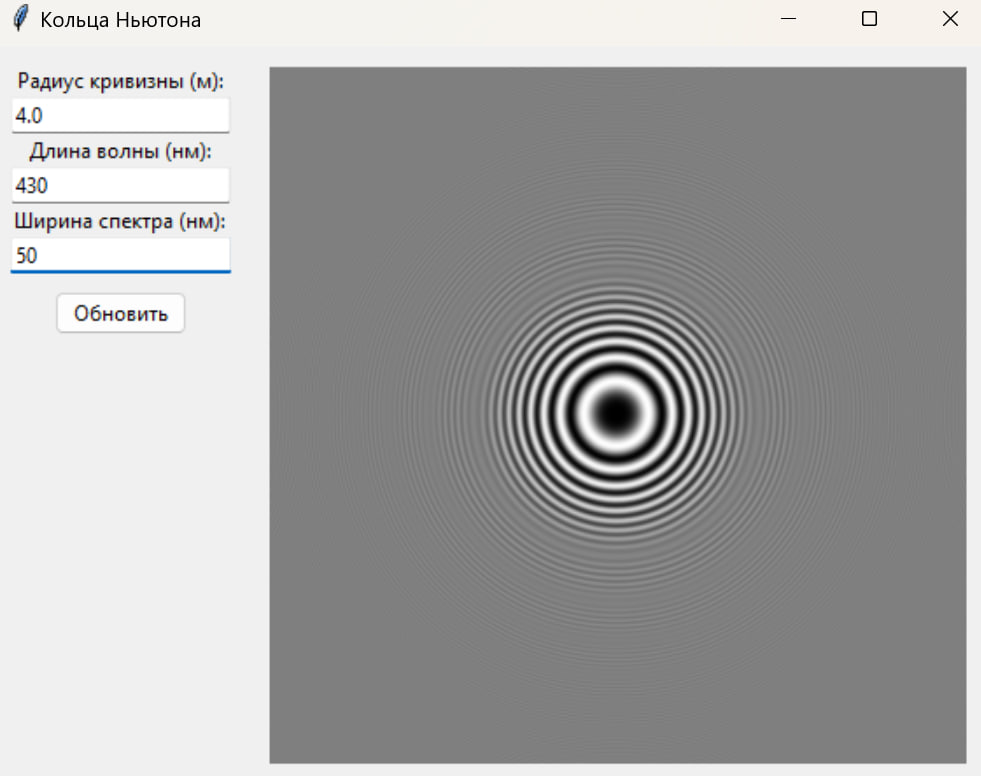
\includegraphics[scale=0.7]{demo results/wideSpectre_quasi}
\end{document}
